
%%%%%%%%%%%%%%%%%%%%%%% file typeinst.tex %%%%%%%%%%%%%%%%%%%%%%%%%
%
% This is the LaTeX source for the instructions to authors using
% the LaTeX document class 'llncs.cls' for contributions to
% the Lecture Notes in Computer Sciences series.
% http://www.springer.com/lncs       Springer Heidelberg 2006/05/04
%
% It may be used as a template for your own input - copy it
% to a new file with a new name and use it as the basis
% for your article.
%
% NB: the document class 'llncs' has its own and detailed documentation, see
% ftp://ftp.springer.de/data/pubftp/pub/tex/latex/llncs/latex2e/llncsdoc.pdf
%
%%%%%%%%%%%%%%%%%%%%%%%%%%%%%%%%%%%%%%%%%%%%%%%%%%%%%%%%%%%%%%%%%%%

\documentclass[sigchi]{acmart}
% Removes citation information below abstract
\settopmatter{printacmref=false} 
% removes footnote with conference information in first column
\renewcommand\footnotetextcopyrightpermission[1]{} 
\pagestyle{plain} % removes running headers

%%%% PACKAGES
\usepackage[T1]{fontenc}
\usepackage{lmodern}
\usepackage{booktabs} % For formal tables
\settopmatter{printacmref=false}
\setcopyright{none}
\usepackage{subcaption}
%\usepackage{amssymb}
%\setcounter{tocdepth}{3}
%\usepackage{graphicx}
%\usepackage{enumerate}
%\usepackage{url}
%\usepackage{comment}
%\usepackage[draft]{todonotes} 
%\usepackage{changes}

\usepackage[T1]{fontenc}
%Conference
%% DOI
%\acmDOI{10.475/123_4}
%
%% ISBN
%\acmISBN{123-4567-24-567/08/06}
%
%%Conference
%\acmConference[WOODSTOCK'97]{ACM Woodstock conference}{July 1997}{El
%	Paso, Texas USA} 
%\acmYear{1997}
%\copyrightyear{2016}
%
%\acmPrice{15.00}
%
%\acmSubmissionID{123-A12-B3}


\begin{document}

%%% TITLE SECTION
\title{Machine Learning Models for Dynamic Product Repricing on the Amazon Marketplace}
\titlenote{This project has been funded by SFI award IP/2016/0436}
\keywords{Dynamic Repricing, Amazon Marketplace, E-Commerce, BuyBox Prediction, Machine Learning}


%%% AUTHOR SECTION
\author{Thanh-Binh Le, Georgiana Ifrim}
%\authornote{Insight Centre for Data Analytics, University College Dublin, Ireland}

\affiliation{%
	\institution{Insight Centre for Data Analytics, University College Dublin, Ireland}
}\email{{thanh.binh, georgiana.ifrim}@insight-centre.org}

\begin{abstract}	
	
	E-commerce has grown hugely and has opened opportunities for retailers big and small to sell their products on online shopping platforms such as the Amazon Marketplace. The Amazon platform hosts thousands of retailers and uses an algorithmic decision process called the BuyBox, to decide which product offer to show first in return to a user query.

	Every time the price of a product changes, an auction among all the competing offers for that product takes place, and the BuyBox winner is re-assigned by Amazon. The BuyBox winner typically sells more products and achieves a higher revenue. The price of a product plays a large role, but it is not the only indicator of an offer winning the BuyBox. If we can understand and accurately approximate the BuyBox assignment algorithm, we can advise sellers about how to best customise their offers. We can also employ the same algorithm for dynamic repricing of products, to increase the likelihood of an offer winning the BuyBox, in the context of continuous change in competing offers.
	
	Most existing solutions for predicting the BuyBox and for product repricing are closed commercial solutions. In this study we analyse historical data describing thousands of Amazon BuyBox auctions  and build machine learning models that aim to approximate the Amazon algorithm for selecting winners. We also investigate approaches for algorithmic re-pricing based on (1) our BuyBox prediction algorithm and (2) efficient price point search strategies. Our evaluation shows that our learning models can accurately predict the BuyBox winner and can recommend effective repricing strategies.
	%\keywords{Dynamic Repricing, Amazon Buybox, Business E-Commerce, Random Forest Classifier, Feature Impotance}
 
	
\end{abstract}

\maketitle


%%% MAIN SECTIONS
%!TEX root = main.tex
\section{Introduction}
\label{sec:introduction}

%% Begin the state (edited)	
Nowadays, the rise of e-commerce has opened many opportunities and challenges 
for merchants to sell their products and re-act their selling immediately. 
The on-line marketplace such as Amazon, provide many supporting tools to sellers 
that they can supervise their products at any given point of time. 
On the one hand, Amazon helps the merchants to adapt their product's 
price effectively in order to gain their profit. On the other hand, it also increases 
much pressures to the retailers, who have limited experience with such highly
competitive markets and their long-term effects. To deal with that concern, the sellers 
use dynamic pricing tools to adjust product prices and manage inventories in real-time. 

%% What is Dynamic pricing
Dynamic pricing is the study of determining optimal selling prices 
of products or services, in a setting where prices can easily and 
frequently be adjusted. This applies to vendors selling their 
products via Internet, or to brick-and-mortar stores that make use 
of digital price tags. In both cases, digital technology has made it 
possible to continuously adjust prices to changing circumstances, 
without any costs or efforts. Dynamic pricing techniques are nowadays 
widely used in various businesses, and in some cases considered to be 
an indispensable part of pricing policies. Digital sales environments 
generally provide firms with an abundance of sales data.

%% Talk about the key points
This data may contain important insights on consumer behavior, in 
particular on how consumers respond to different selling prices. 
Exploiting the knowledge contained in the data and applying this to 
dynamic pricing policies may provide key competitive advantages, 
and knowledge of how this should be done is of highly practical relevance 
and theoretical interest. This consideration is a main driver of 
research on dynamic pricing and learning: the study of optimal 
dynamic pricing in an uncertain environment where characteristics 
of consumer behavior can be learned from accumulating sales data. 

%% What is challenging?
More recently, research and industry started to combine
achievements of price optimization from the research field
of operations research with the achievements in data-driven
procedures from the field of computer science such as machine
learning. This development is basically catching-up
with similar approaches already being applied in the field
of algorithmic trading or high-frequency trading on stock
exchanges. These approaches are far more sophisticated than
currently observable approaches on marketplaces such as
Amazon, where most merchants thrive to be amongst the
cheapest competitors, eventually leading to a typical race to the
bottom. 
%More sophisticated strategies optimize for long-term
%profits, consider restocking, and predict competitor actions.
%Unfortunately, for practitioners as well as for researchers,
%a common platform to develop, test, and evaluate pricing
%strategies is missing. Merchants lack the possibility to test
%their strategies appropriately before deploying them in production,
%potentially causing significant economic problems. For
%researchers, there are no open platforms for simulating large
%pricing competitions with various pricing strategies competing
%with each other. More importantly, there are no platforms that
%provide the means to deploy data-driven strategies.

%% What is our contribution
The Amazon Online Marketplace is the largest and fastest growing 
retailer marketplace, with more than 3 million retailers selling products on this platform \cite{}. 
Amazon constantly ranks the sellers based on different attributes, 
such as product price, customer satisfaction, amount of transactions completed, etc., and presents the best ranked seller/offer in the BuyBox. 
Pricing is the the most influential factor short-term to rank at the top, but the other attributes describing the seller and the offer are also important (e.g., shipping time, 
stock available).
Existing repricing solutions use seller-provided rules for updating the product price when a repricing event is triggered 
(e.g., update price by 1\% when a competitor changes the price of a product). 
These fixed rules are set manually and changed infrequently based on a schedule decided by the seller.

A Machine Learning solution for dynamic repricing can take full advantage of past 
detailed historical data about competing offers and the outcome of auctions, and should remove the need 
for slow to update and potentially non-optimal manual-rules.
This can result in optimised pricing decisions for the sellers which should rank them top 
on the sales platform consistently, therefore laying the foundation for increased sales and better competitiveness.
%to existing customers and a strengthened value proposition to attract new customers.
Additionally, the insights derived from analysing the historical data and the resulting predictive models should allow sellers 
to adapt to ever changing market conditions beyond pricing. 
%This will result in a deep understanding of parameters, which may result in introducing new parameters or adapting multiple parameters to gain the best result for the customers. 
%This may also lead to additional consulting opportunities for XSellco.
%Solution / Product
%Briefly describe what the team hope to produce from the partnership.
%This project aims to develop scalable Machine Learning methods that can automatically recommend appropriate product repricing, by taking into account historical and dynamic data describing the retailer, the product, the competitor products, demand, etc. A learning approach is needed to automatically infer patterns from dynamic and vast historical data, without the need for human-built rules that do not make the best use of the data available.
%The learning model aims to be accurate and scalable, to be able to deal with millions of repricing events which are constantly changing. The predictive model also aims to be interpretable, so the insights learned from the model can be used by XSellco to offer additional consulting.
%To start with, the project has historical data available from XSellco about thousands of retailers and products, as well as repricing event details from 2013 to today. This data will be used to build predictive models that describe the relationship between data and desired outcomes, such as winning the Amazon ?Buy Box? at the price that maximises profit for the retailer.

In this work we have access to large amounts of auction data 
for products sold over the course of 9 months on the Amazon Marketplace. 
Our aim is to develop machine learning algorithms to predict the BuyBox winner, as well as study  
dynamic repricing strategies for individual sellers.

Our key contributions are as follows:
\begin{itemize}
\item \textbf{Data Preparation Techniques:} We present data pre-processing and preparation techniques suitable for product auction data collected from the Amazon Marketplace, with a view to 
build effective BuyBox prediction algorithms. 
\item	\textbf{BuyBox Predictor Algorithm:} We propose a machine learning algorithm that can be trained on historical product auction data from the Amazon Marketplace, 
and can be used to predict the winner of a new auction on the Amazon Marketplace (i.e., BuyBox winner predictor). 
Our algorithm is based on a RandomForest classifier that uses carefully engineered features.
We also discuss the importance of different features for predicting the BuyBox.

\item \textbf{Repricer Algorithm:} We implement and evaluate a dynamic repricing algorithm that can take in an auction for a given product and seller, 
and recommend a repricing strategy to maximise the probability of winning the next auction for that seller and product.
Our algorithm is based on the BuyBox predictor model and on a strategy for selecting candidate price points for recommendation.

\item \textbf{Evaluation/Deployment:} All our algorithms are tested on research benchmarks and are deployed on commercial platforms.
We discuss the results and what we learn from deploying our algorithms.
\end{itemize}

%-------------------------------------------------------------------------

\section{Related Work}
\label{sec:RelatedWork}



%%------------------------------------------------------------------------
%

\section{Background}
\label{sec:Background}
In this section, we first briefly introduce the Amazon Marketplace. Then, we focus on the data features on the markets, that effect to algorithmic repricing, including the offers of 3P merchants, the BuyBox concept, and finally the scaled data, collected from the Amazon Web Services (AWS).

\subsection{The Amazon Marketplace}
\label{sec:amzintro}
%% Talk a bit about Amazon online marketplace
The Amazon Marketplace is one of the most well-known marketing channels for online retailers. 
It is an e-commerce platform, which enables  sellers to sell their products on its cloud markets. 
Started as a book seller but later Amazon (amazon.com) has expanded to sell varied categories of consumer 
items as well as its own electronic machinery. The Amazon has separate marketplaces for the United States, 
Australia, Brazil, Canada, China, France, Germany, India, Italy, Japan, Mexico, Netherlands, Spain, and the United Kingdom.

In 2015, Amazon surpassed Walmart to be the most valuable retailer in the United States \cite{kantor2015inside}. 
In 2017, it becomes one of the top 10 world's largest online marketplace with around 80 million worldwide members 
(refered to \textit{"Global Powers of Retailing 2017"} report {\footnote{\url{https://www2.deloitte.com/
content/dam/Deloitte/global/Documents/consumer-industrial-products/gx-cip-2017-global-powers-of-retailing.pdf}}). 
In the same year, the using Amazon mobile application also reached the peak of 41.50\% to become the top most 
popular mobile shopping app in the United States, this is illustrated by \textbf{Fig.\ref{fig:statistic}} 
(refered to www.statista.com {\footnote{\url{https://www.statista.com/statistics/579505/most-popular-
us-shopping-apps-ranked-by-reach/}}}). 

\begin{figure}[!h]
	\begin{center}
		\scalebox{0.27}{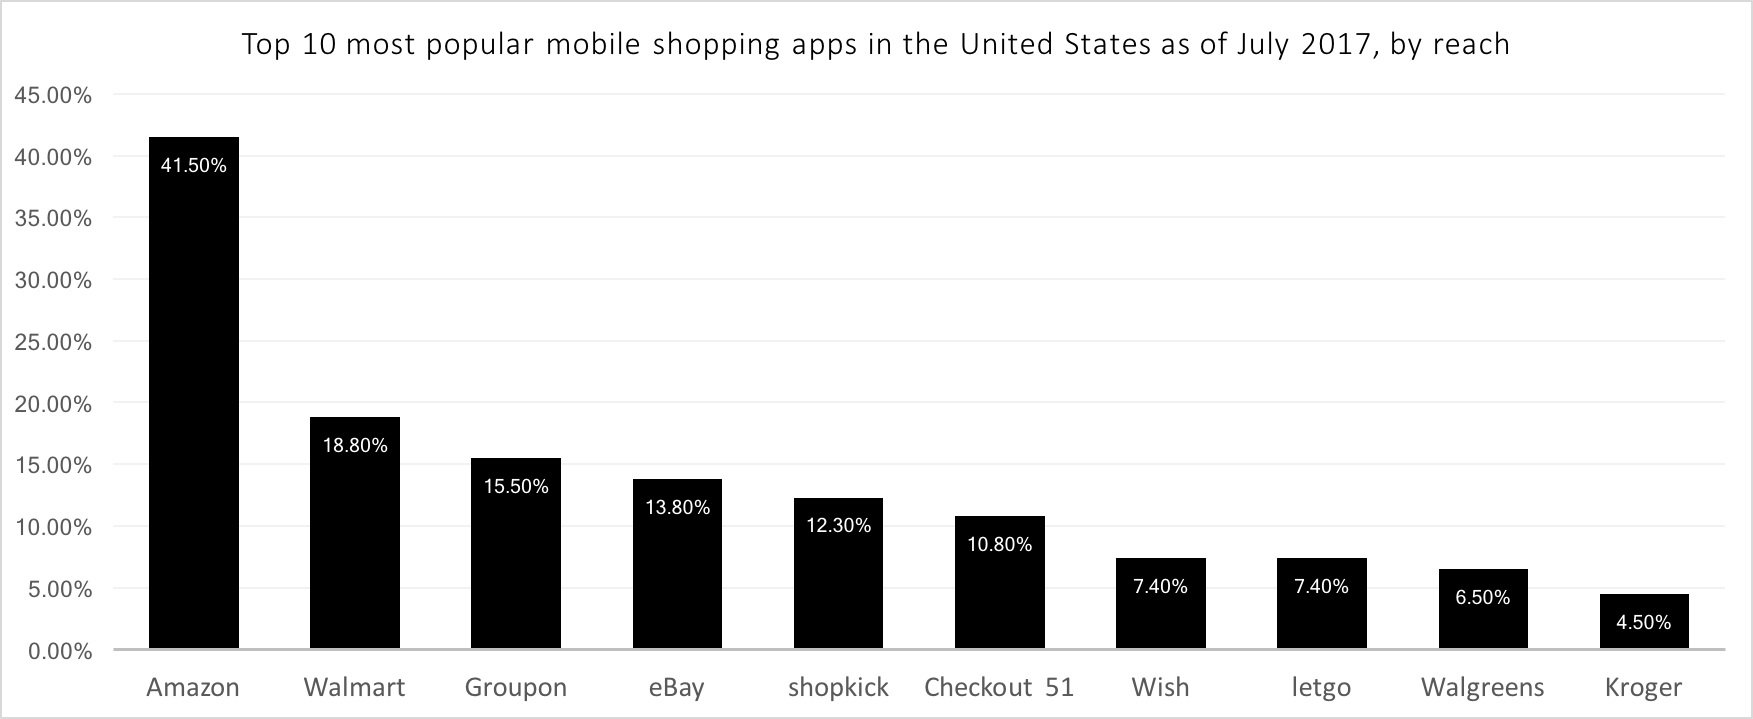
\includegraphics{fig6_statisticAMZ.png}}
	\end{center}
	\caption{\label{fig:statistic} Top 10 of most popular mobile shopping apps in the United States as of July 2017, by reach.}
\end{figure}
%%Talk more about amazon
%% FBA and FBM
%Goods purchased on Amazon from  sellers are either fulfilled by the merchant (FBM) or by Amazon (FBA). FBM sellers must keep items in their inventory, and must manage their shipping and customer service. Perversely, FBA sellers can store the goods in Amazon's fulfillment centers, while shipping and customer services are organized by Amazon. 

%% Amazon fee -> need to take advantage from repricing
%There are several Selling Fees for  retailers to put their products on Amazon Marketplace, including:
%\begin{enumerate}
%	\item \textbf{Per-item Fee}: When one product sells, Amazon collects the amount paid by the buyer (\$0.99/item sold, or sellers may become “Pro Merchants” with no fee)
%
%	\item \textbf{Referral Fee}:  sellers have to pay a referral fee on each product sold. The referral fees vary by category between 6\%-45\% of the total sale price. However, the enforcement of minimum referral fees is \$1-\$2/item.
%
%	\item \textbf{Closing Fee}: For each media product that is sold, Individual and Professional Sellers also pay a variable closing fee (\$1.80 per media product).
%
%	\item \textbf{High-Volume Listing Fee}: Amazon charges a monthly High-Volume Listing Fee based on the number of active offers for non-media products listed on Amazon (\$0.005 per product).
%
%	\item \textbf{Refund Administration Fee}: It is the lesser of \$5.00 or 20\% of the applicable Referral Fee if a seller refunds a customer for an order for which that seller has already received payment.
%\end{enumerate}

%\subsubsection{Third-party Sellers and FBA}. In addition to acting as a merchant, Amazon also functions as a marketplace for third parties. Amazon claims to have 2M Third-Party () sellers worldwide who sold 2B items in 2014, representing 40\% of all items sold via the website.  sellers can opt to handle logistics (inventory, shipping, returns, etc.) themselves, or they can join the Fulfilled By Amazon (FBA) program, in which case Amazon handles all logistics.

\subsection{The BuyBox}
\label{sec:buybox}
%% What is winner BuyBox?
The Amazon BuyBox is definitely the most important element to sellers in Amazon Marketplace. 
It is the box from the right of the product page which contains the \textit{"Add to Basket"} 
or \textit{"Add to Cart"} button. \textbf{Fig.\ref{fig:buyboxexample}}, an example BuyBox, 
shows that winning the BuyBox is critical for generating sales. The BuyBox contains the price 
of the product, shipping information, the name of the seller, and a button to purchase the product.
 When customers click the button, they are buying the product from only one merchant who is the BuyBox 
 winner. The winner gets more chance to sell their items by getting the prominent position in product's 
 page , while the other competitors are relegated to the bottom section with a lower priority. Amazon 
 themselves admit that around 82\% of purchases are made through the BuyBox \cite{taftamazon}. 

\begin{figure}[!h]
	\begin{center}
		\scalebox{0.40}{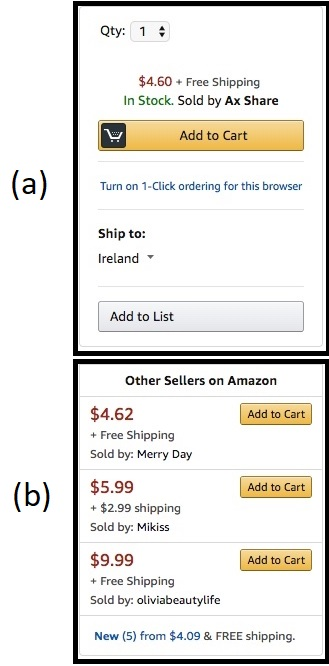
\includegraphics{fig1_buybox.png}}
	\end{center}
	\caption{\label{fig:buyboxexample}In the Amazon's product page, the products of the BuyBox 
		winner can be highlight effectively in the BuyBox (a), while the other competitors get lower 
		positions (b).}
\end{figure}


%% Why is it important?
However, multiple sellers can offer the same product in Amazon Marketplace. If more than one eligible seller offers a product, they may compete for the BuyBox position. \textbf{Fig.\ref{fig:exampleoffer}} is an example of one product's auction provided by many competitors with different information, prices, deliveries, and conditions. Every time one seller changes the price of a their product, the BuyBox winner is re-assigned by Amazon. 

Amazon has a convoluted algorithm to determine which seller gets the prime location on the BuyBox. Understanding the BuyBox algorithm is essential, because it may help sellers choose better pricing strategies for their next auctions.  Amazon has a notation about the features which are used by the BuyBox algorithm \cite{amazon17}, but it is uncertain whether the feature list is complete, or what the important weights of the features are. Because winning the BuyBox is so critical for making sales on Amazon,  sellers may use dynamic pricing strategies that give them an advantage to be chosen by the BuyBox algorithm.

\begin{figure}[!h]
	\begin{center}
		\scalebox{0.25}{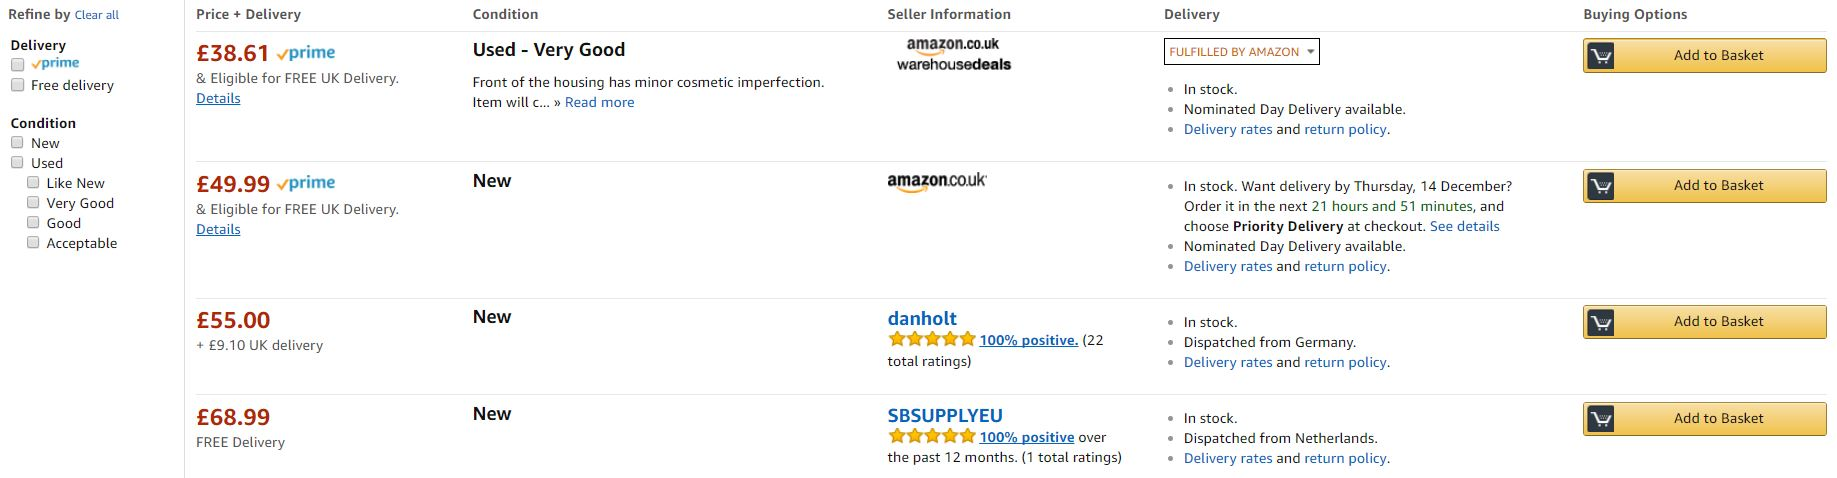
\includegraphics{fig2_offers.JPG}}
	\end{center}
	\caption{\label{fig:exampleoffer}An example of the offers for one product item on Amazon with many different competitors.}
\end{figure}

%\subsection{Data Understanding}
%\label{sec:DataUnderstanding}

%% how to get data?
\subsection{Amazon Web Service (AWS)}
\label{sec:awsData}
%% definition
 Amazon offers an array of tools to help sellers manage product selling. The most knowing of these tools is the Amazon Marketplace Web Service (MWS). Amazon Web Services (AWS) is a bundled remote computing service that provides cloud computing infrastructure over the Internet with storage, bandwidth and customized support for application programming interfaces (API).

From AWS, users has a capability to control their product updates for specified products from the Amazon cloud service. They are able to acknowledge their current state in the price-battle competed to their competitors. They can know who is the buy box winner, how many offers are provided by their competitors ... They also can execute several tasks through the provided functions such as listing products, managing inventory, and changing prices. 

The data from AWS can be pulled using the XML format, and then it can be parsed and stored into comma-separated value (CSV) file. Each row in the CSV file is a single data record or observation of one seller in the product's competition. Each column in the CSV contains a attribute of offers. 
%Its value is manually set by the seller or it is automatic defined by Amazon.


\subsection{Competition Auction}
\label{sec:amzAuction}

From mentioned above, the AWS helps users control their selling, including updating prices for their products. Whenever one seller changes or updates their offer for one item, AWS keeps a new record for that update with fully information for the lowest 20 prices offered of that product item (or less, if there are fewer than 20 offers). Since one auction happens, then one new XML is created from AWS.

% \section{Data Understanding}
\label{sec:DataUnderstanding}

%In this section, we provide the details of Amazon Data. In particularly, sub-section \ref{sec:amzScale} will describe the scaling of amazon data, section \ref{sec:featureunderstanding} will summarize the useful features of data. 

\subsection{Amazon Data Scale}
\label{sec:amzScale}

% Scale of amazon data
As mentioned above, every changing for a customer's offer in product page is stored by an auction xml file. An auction includes aggregated information about the lowest 20 prices offered for a product (or less, if there are fewer than 20 offers).  \textbf{Fig.\ref{fig:scale}} illustrates the scaling of data in one market. It is provided from several layers as follows:

1. \textbf{Marketplace's scale layer}: The Amazon has many marketplaces for
the United States, Australia, Brazil, Canada, China, France, Germany, India, Italy, Japan, Mexico, Netherlands, Spain, and the United Kingdom. One marketplace is an separated  environment with its own characteristics.  e.g. in India market, there is one seller who wins almost product's competing, while in U.S. market, the auction is normally with two or three competitors.

2. \textbf{Product's scale layer}: From the market place, sellers can sell many products. It could be very different in price, shipping time, conditional note for two different products. The category list of product can be found in the Amazon Web Service.

3. \textbf{Auction's scale layer}: In product's layer, the auction can be recorded when sellers update their product's offers. For example, one seller changes their shipping time from 0 hour to 24 hours, the new auction of that changing with all information of its competitors is parsed as one new XML.

4. \textbf{Offer's scale layer}: One auction contains many offers of sellers in one product. They could be old or new updated offers.


\begin{figure}[!h]
	\begin{center}
		\scalebox{0.5}{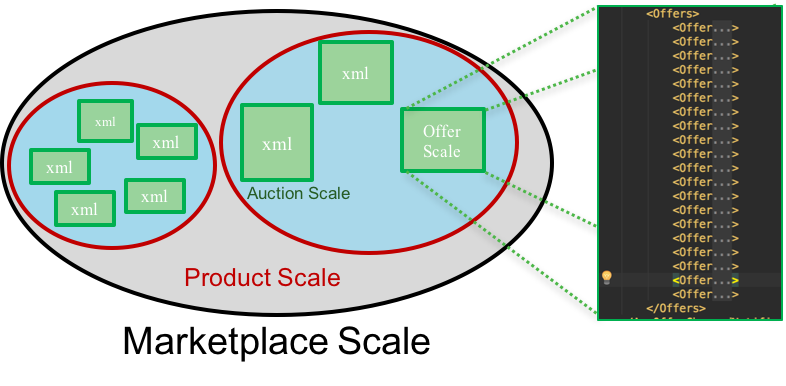
\includegraphics{fig3_scale.png}}
	\end{center}
	\caption{\label{fig:scale}The scales of data in one Marketplace.}
\end{figure}

\subsection{Features Understanding}
\label{sec:featureunderstanding}

%% table of features


%% New feature
To facilitate the analysis, we model the Buy Box as a prediction problem. Specifically, for a product offered by $n$ sellers, each of which is characterized by a feature vector, our goal is to predict which seller will be chosen to get in the Buy Box. Given the list of XMLs, we create a feature vector for each seller containing the following seven features:

1. xxx

2. xxxx

3. xxxx

4. xxxx

According to Amazon’s documentation, as well as speculation from 3P sellers, other
features are possibly used by the Buy Box algorithm [11, 31]. This includes sales volume, response time to customer inquiries, rate of returns and refunds, and shipping times. Unfortunately, I cannot measure these features, and thus cannot quantify their impact on the Buy Box algorithm. However, as I will show, even without these features I am able to achieve high prediction accuracy, suggesting that my data does capture the most important seller features.

\begin{figure}[!h]
	\begin{center}
		\scalebox{0.27}{\includegraphics{fig7_fi.png}}
	\end{center}
	\caption{\label{fig:fi}An example of the Feature Importance, provided by Random Forest classifier.}
\end{figure}

\section{BuyBox Prediction}
\label{sec:buybox}
% This is the brief introduction of our goal in this section
This section provides a machine learning algorithm which can take as input any dataset describing the offers made by sellers for a set of products, for a specific market (e.g., US, UK, France) or across markets. It then trains a machine learning model that, when presented with an auction, it can predict the offer that will win the auction (BuyBox). The algorithm also outputs a ranked list of the feature importance discovered from the training data. For example, the algorithm can discover data-specific feature importance for each input dataset. This means that the algorithm can be targeted to the data of a single seller or a specific product, and it delivers a list of feature importance for that custom data. So besides predicting the auction winner, the algorithm can be used to advise sellers on how best to update their offer profiles to increase their chance of winning the BuyBox.

\subsection{Business Understanding}
\label{sec:bbbusiness}
%% our target in increasing profit by placing offer into BuyBox
Amazon hosts thousands of  sellers on their marketplace. They use an algorithmic decision process to decide the winner of every auction. An auction as mentioned above is a set of merchants that compete to sell a product. Amazon selects a winner for the auction, and place that seller's product into the BuyBox. The BuyBox winner typically sells more products, and ideally achieves a higher profit margin. This means that the winner is highly competed by many retailers in auction.

Motivated by that, our target is clearly declared as: can we use historical data about auctions and knowledge about the winners and losers, to learn the rules by which Amazon decides the winners? If we can approximate Amazon’s algorithm, we can advise sellers about the best strategy to use for winning the BuyBox. For example, we can recommend a new price for the product, or give advice about shipping time and user feedback profile to improve the offer and increase the chance of winning the BuyBox. 

\subsection{Data Understanding}
\label{sec:datafirstlook}
% Scale of amazon data
As mentioned above, every changing for a seller's offer detail in product page provides an auction, in AWS cloud. It includes aggregated information about the 20 lowest prices offered for a product (or less, if there are less than 20 sellers). Each auction is represented as a XML, the total size of raw-data folder, which is a cross-market database, is about 100.000 files. 
\begin{figure}[!h]
	\begin{center}
		\scalebox{0.5}{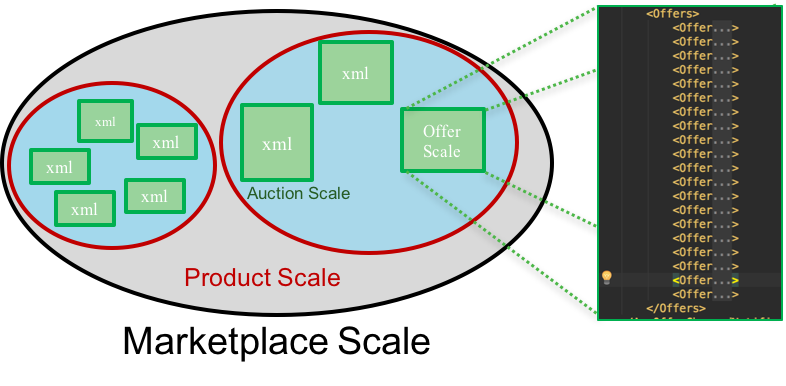
\includegraphics{fig3_scale.png}}
	\end{center}
	\caption{\label{fig:scale}The scales of data in one Marketplace.}
\end{figure}

Illustrating from \textbf{Fig.\ref{fig:scale}},which is the scaling scheme of data in one market, there are four basic layer for the Amazon data:

1. \textbf{Marketplace layer}: The Amazon has many marketplaces for
the United States, Australia, Brazil, Canada, China, France, Germany, India, Italy, Japan, Mexico, Netherlands, Spain, and the United Kingdom. One marketplace is an separated  environment with its own characteristics.  e.g. in India market, there is one seller who wins almost product's competing, while in U.S. market, the auction is normally with two or three competitors.

2. \textbf{Product layer}: From the market place, sellers can sell many products. It could be very different in price, shipping time, conditional note for two different products. The category list of product can be found in the Amazon Web Service.

3. \textbf{Auction layer}: In product's layer, the auction can be recorded when sellers update their product's offers. For example, one seller changes their shipping time from 0 hour to 24 hours, the new auction is saved as one XML file.

4. \textbf{Offers layer}: There are many  sellers give their offer for a product in marketplace. However, only the 20 lowest price offers are saved in XML when an auction is happened.

\subsection{Data Preparation}
\label{sec:dataprepare}

\subsubsection{Raw Data:}
\label{sec:datacsv}
%% Features list and description
To facilitate the analysis, we model the BuyBox as a prediction problem. Specifically, for a product offered by $n$ sellers, each of which is characterized by a feature vector, our goal is to predict which seller will be chosen to get in the Buy Box. 

First step is to parse the XML raw data files into a single CSV dataset that can be use for further data analysis. We do this by parsing every single XML file, and turning each tag in the XML file, into a row of the CSV file. This row describes the features of an offer and the target feature is the \textbf{IsBuyBoxWinner} (which is 1 if the offer in BuyBox, -1 otherwise). All the offers under the tag \textbf{<Offers>} become rows in the CSV file. Since each XML file has up to 20 offers, this means that for each auction we generate up to 20 rows in the CSV file. Each Offer tag becomes a row in the CSV file, and each tag or subtag, becomes a column name. We give details below for the number of rows and columns generated by parsing over 100k XML files.

The feature vector is described into four categories as follows :

\textbf{1. Prices}: The price's features are related to the price of products, which customers have to pay for buying a product. They are the \textit{ListingPrice} and \textit{ShippingPrice}. In addition, the new feature \textit{LanddedPrice} = \textit{ListingPrice} + \textit{ShippingPrice} is also calculated.

\textbf{2.Shipping Time Informations}: These are the shipping details for one seller's product, including the \textit{ShippingTime\_minHours}, \textit{ShippingTime\_maxHours} for delivery. 

\textbf{3. Seller Feedback Information}: These features describe the detail of seller's feedback, including feedback's counts (\textit{SellerFeedbackCounts}) and feedback's rating (\textit{SellerFeedbackRating}). 

\textbf{4. Retailers' Details}: These features are the basic detail of  sellers when they have a cooperate to Amazon. These features denote whether the seller is fulfilled by Amazon (\textit{IsFulfiledByAmazon}) or by merchant (\textit{IsFeaturedMerchant}). The last feature is the product's condition notes \textit{ConditionNotes} from sellers to their buyers.

\subsubsection{Data Analysis:}
\label{sec:dataanalysis}

%% talk a bit about the correlation between features in each market ==> need to prvide the solution 
%% by each market
After parsing data into CSV format, the features are analyzed to help us having a clear understanding. Our first concern is about whether we can use data from cross-market to learn model. By observation \textbf{Fig.\ref{fig:corr}}, it clearly shows that we should not train model with cross-market data. The correlations between features of two markets are really different, e.g. the possibility to be in BuyBox is higher if we have smaller shipping times in U.S. market, while it is not a really strong concerned effect in U.K. market. %In U.K. shipping time is not the big anxiety for the buyers. 
Hence, the separated treatment for each marketplace is necessarily provided.

\begin{figure}
	\begin{subfigure}{0.45\textwidth}
		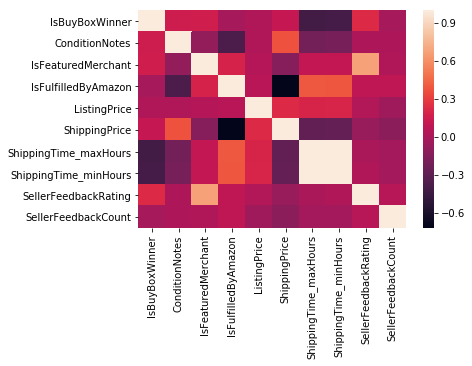
\includegraphics[width=\linewidth]{fig_market_US_corr.png}
		\caption{The U.S. \textit{"amazon.com"} market } \label{fig:corrus}
	\end{subfigure}
%	\hspace*{\fill} % separation between the subfigures
	\begin{subfigure}{0.45\textwidth}
		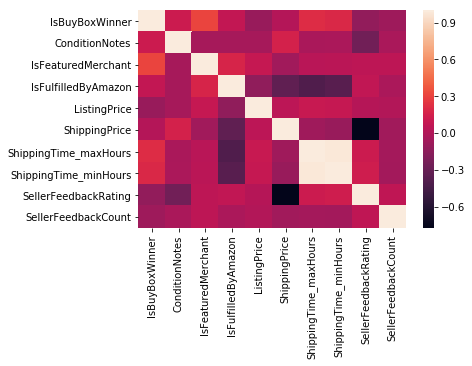
\includegraphics[width=\linewidth]{fig_market_UK_corr.png}
		\caption{The U.K. \textit{"amazon.co.uk"} market} \label{fig:corrfr}
	\end{subfigure}
	\caption{The correlation between features in (a) U.S. market and (b) U.K. market.} \label{fig:corr}
\end{figure}

In addition, we create some new features to enrich the information of an auction. These features are described as follows:

\textbf{1. Difference to Minimum Price in Auction}: (\textit{DifftoMinLandedPriceCompetition})This is the difference from current LandedPrice to the minimum landed price in that auction.

\textbf{2. Difference to the Minimum Price of Product}: (\textit{DifftoMinLandedPriceProduct}) This is the difference from current LandedPrice to the minimum landed price, grouped by product.

\textbf{3. Difference to the Amazon Seller's Price}: (\textit{DifftoAmzLandedPriceCompetition}) We capture who is the Amazon Seller in the auction. Then, we calculate the difference from current LandedPrice to the Amazon Price. If there is not Amazon Seller in the auction, we use the difference to minimum price in the auction instead.

\textbf{4. Difference to the Ideal Point in Auction}: (\textit{IdealPointCompetition}) The ideal point is the combination between the best (i.e., minimum) LandedPrice and the best (i.e., minimum) ShippingTime\_maxHours, across all offers, in each auction. This feature captures the difference from this ideal point, for each offer in the auction.
\begin{figure}[!h]
	\begin{center}
		\scalebox{0.28}{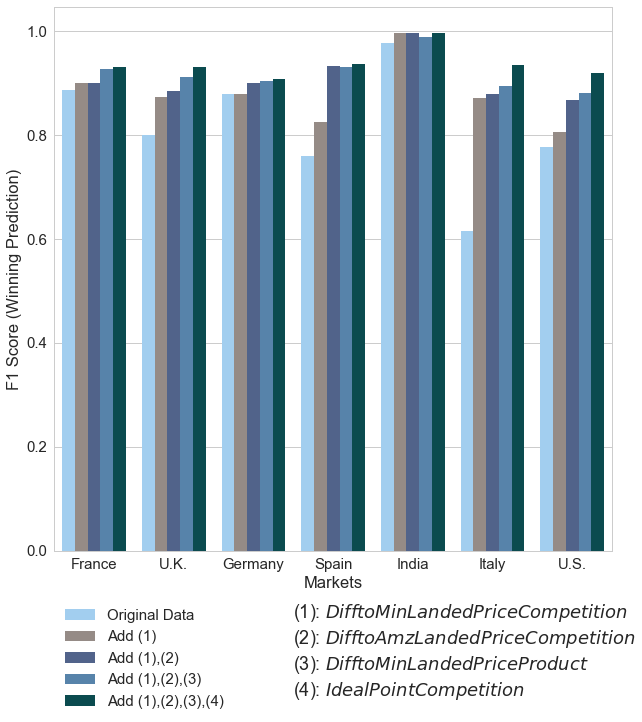
\includegraphics{fig_addFeatures.png}}
	\end{center}
	\caption{\label{fig:addfeaures}A comparison of F1-score when predicting winner BuyBox for 7 marketplaces. The scores are provided by Random Forest classifier.}
\end{figure}

%\subsubsection{Feature Selection:}
%\label{sec:featsel}
%%% This will talk about the feature importance?
%According to Amazon's documentation, as well as speculation from sellers, other
%features are possibly used by the Buy Box algorithm. 
%
%\begin{figure}[!h]
%	\begin{center}
%		\scalebox{0.27}{\includegraphics{fig7_fi.png}}
%	\end{center}
%	\caption{\label{fig:fi}An example of the Feature Importance, provided by Random Forest classifier.}
%\end{figure}

In order to check the model's improvement capability for the new features, we add those features one after another and compare them with the F1-scores by using Random Forest Classifier. \textbf{Fig.\ref{fig:addfeaures}} illustrates that the prediction becomes better when adding the extra information. This upgrading also points that the new features can enrich the Amazon data and help to build a better hypothesis.


\subsection{Machine Learning Model for Predicting BuyBox Winner}
\label{sec:buyboxmodel}

In here, we introduce the model construction with BuyBox Predictor. The goal of this algorithm is to predict the probability to win buy box. From parsed data, we use the Random Forest classifier to build the R.F. tree, which has information of who is winner and who can never win. The \textbf{Fig.\ref{fig:buyboxflow}} shows the flowchart of BuyBox prediction algorithm.

\begin{figure}[!h]
	\begin{center}
		\scalebox{0.70}{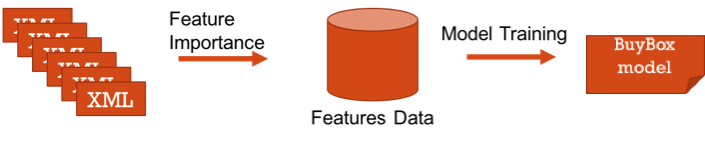
\includegraphics{fig4_buybox.png}}
	\end{center}
	\caption{\label{fig:buyboxflow}The flowchart of BuyBox model for winner prediction using feature importance to rank and select best features.}
\end{figure}

\subsection{Experiment for Predicting BuyBox Winner}
\label{sec:expbuyboxmodel}



\begin{center}
	\begin{table}[htb]
		\label{exp:prediction}
		\begin{tabular}{ |c|c|c|c|c|c|c|c|c|c|c|c|c|c| } 
	
	
			\specialrule{.2em}{.1em}{.1em} 
			\multirow{2}{*}{Markets (Sample size)} & \multirow{2}{*}{Class}  & \multicolumn{2}{c|}{R.Forest} & \multicolumn{2}{c|}{L.Regression } & \multicolumn{2}{c|}{3-NN}&  \multicolumn{2}{c|}{AdaBoost} & \multicolumn{2}{c|}{SVM-RBF} & \multicolumn{2}{c|}{XGBoost} \\ \cline{3-14}
			
			& &	 mean &	std	 & mean & std & mean &std & mean & std & mean & std	& mean & std \\ 
			\specialrule{.1em}{.05em}{.05em} 
			\multirow{2}{*}{France (475,612)}	&  -1 &1.000 &0.000 &0.990	&0.000 &0.990 &0.000 &0.990 &0.000 &0.990 &0.000 &0.990 &0.000 \\ 
												&	1 &0.960 &0.004	&0.800	&0.000 &0.860 &0.015 &0.870	&0.005 &0.830 &0.011 &0.900	&0.000 \\ 
			\hline
			\multirow{2}{*}{UK (86)}	&-1	&0.980	&0.019	&0.935	&0.013	&0.950	&0.011	&0.905	&0.011	&0.915	&0.031	&0.980	&0.012 \\ 
										&1	&0.970	&0.022	&0.915	&0.019	&0.940	&0.011	&0.880	&0.014	&0.895	&0.045	&0.970	&0.018 \\ 
			\hline
			\multirow{2}{*}{Germany (113)}  &-1	&0.930	&0.023	&0.940	&0.014	&0.945	&0.024	&0.940	&0.012	&0.930	&0.016	&0.940	&0.012 \\ 
											&1	&0.895	&0.027	&0.910	&0.021	&0.915	&0.031	&0.915	&0.017	&0.905	&0.020	&0.905	&0.017 \\ 
			\hline
			\multirow{2}{*}{Spain (150)}	&-1	&0.955	&0.028	&0.840	&0.004	&0.925	&0.041	&0.795	&0.021	&0.825	&0.020	&0.960	&0.023 \\ 
											&1	&0.925	&0.037	&0.735	&0.024	&0.890	&0.054	&0.665	&0.025	&0.715	&0.050	&0.935	&0.040 \\ 
			\hline
			\multirow{2}{*}{India (36)}	&-1	&1.000	&0.000	&1.000	&0.000	&1.000	&0.000	&1.000	&0.000	&1.000	&0.000	&1.000	&0.000 \\ 
										&1	&1.000	&0.000	&1.000	&0.000	&1.000	&0.000	&1.000	&0.000	&1.000	&0.000	&1.000	&0.000 \\ 
			\hline
			\multirow{2}{*}{Italy (12,506)}	&-1	&0.990	&0.000	&0.960	&0.005	&0.970	&0.005	&0.980	&0.000	&0.970	&0.000	&0.990	&0.004 \\ 
											&1	&0.960	&0.007	&0.830	&0.018	&0.850	&0.013	&0.890	&0.004	&0.850	&0.005	&0.930	&0.007 \\ 
			\hline
			\multirow{2}{*}{US (3,200)}	&-1	&0.950	&0.005	&0.940	&0.007	&0.940	&0.005	&0.940	&0.004	&0.940	&0.005	&0.950	&0.007 \\ 
										&1	&0.910	&0.010	&0.880	&0.009	&0.890	&0.008	&0.885	&0.007	&0.885	&0.010	&0.900	&0.011 \\ 
			\specialrule{.2em}{.1em}{.1em} 	
	
		\end{tabular}
	\caption{The comparison between 6 classification algorithms for BuyBox prediction through 7 markets.}
	\end{table}
\end{center}
%!TEX root = report.tex
\chapter{Repricer Algorithm}
\label{sec:repricer}

\section{Problem Understading}
\label{sec:rpproblem}

One of the main inputs influencing who becomes the auction winner is the price offered by a seller for the product being auctioned. Product prices change dynamically on the Amazon platform, depending on the real-time competition for selling that product (i.e., the competing offers) and manual repricing rules decided by the seller. We aim to automate the repricing strategy to adapt to observed changes in auction behaviour. The repricing strategy helps to maximise the probability of winning the next auction for the given seller/customer and product. 
 
The problem to be solved is: can we use our BuyBox predictor algorithm to dynamically recommend a product price to a given seller (i.e., a dynamic repricing strategy), for a given auction?

This section provides a dynamic repricing tool that uses BuyBox prediction model in Section \ref{sec:buybox}. The repricing algorithm takes in data describing an auction for a given product and a given seller on the Amazon Marketplace, the BuyBox predictor model trained to predict the winner of any auction (a BuyBox winner predictor algorithm) and the data used to train that model. As output, it produces a few candidate price points for the given customer in the auction, ranks the price candidates and selects the top ranked price as a new price recommendation for that customer.

\section{Spliting the Price's Bins}
\label{sec:spliting}

The first problem we have to solve is how to generate the recommended candidate prices.

\section{Finding Recommendation Score}
\label{sec:finalscore}

\section{Proposed Algorithm for Repricer}

\label{sec:repricermodel}


\begin{figure}[!h]
	\begin{center}
		\scalebox{0.70}{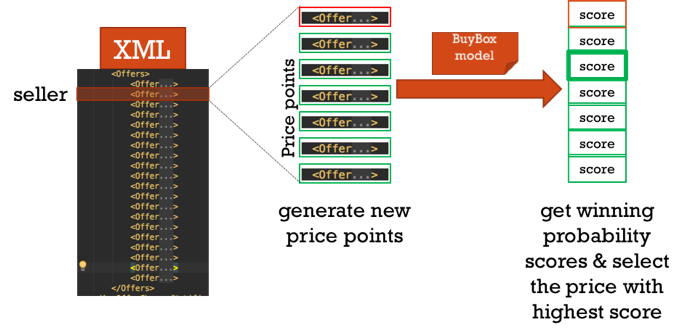
\includegraphics{fig5_repricer.png}}
	\end{center}
	\caption{\label{fig:repricerflow}The flowchart of repricing strategy for one specific seller.
	}
\end{figure}

We provide here the repricing strategy to generate the predictive move of repricing. Our concentration is on the probability of what point of price we can get into buy box with the highest chance we can do. The strategy is defined into three steps:

1) First step is the getting and splitting. We get the point of our customer, who want to make a repricing.
After receive the customer's price, we generate many bins of price, which we would like to test the probability. 

2) Second step is the applying model and generating prediction score. On this step, we apply the Random Forest model, which is learned in BuyBox Predictor. Then we calculate the final scores of all price's points.

3) Final step is selecting. The top 10 largest scores, which has the highest probability to occupy the buy box, is provided as recommended price points. 


\section{Experiment for Repricing}
\label{sec:exprepricer}



\begin{figure}[!h]
	\begin{center}
		\scalebox{0.60}{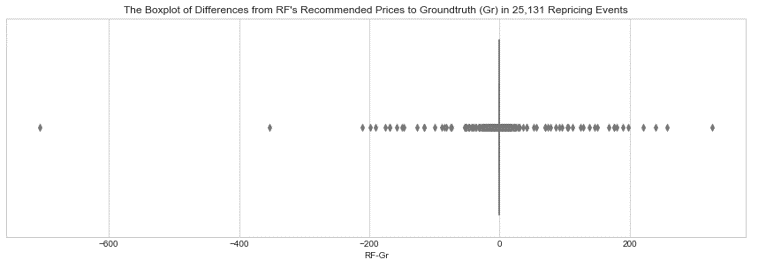
\includegraphics{fig_Boxplot_WinCase.png}}
	\end{center}
	\caption{\label{fig:lostcase}The Box plot of Prediction for Winning Cases.}
\end{figure}


\begin{figure}[!h]
	\begin{center}
		\scalebox{0.60}{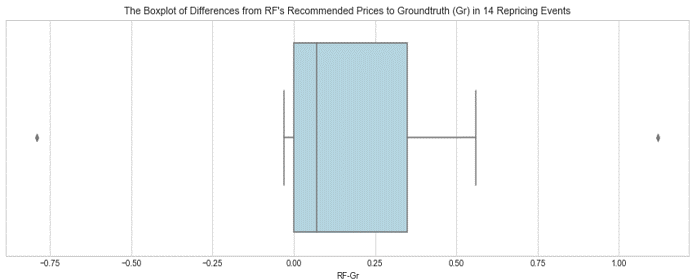
\includegraphics{fig_Boxplot_LostCase.png}}
	\end{center}
	\caption{\label{fig:lostcase}The Box plot of Prediction for Losing Cases.}
\end{figure}
%\section{Evaluation}
\label{sec:Evaluation}

\subsection{BuyBox Winner Prediction Algorithm Evaluation}
\label{sec:BuyBoxEvaluation}

\subsection{Repricing Algorithm Evaluation}
\label{sec:RepricingEvaluation}
%!TEX root = report.tex
\chapter{Conclusion}
\label{sec:Conclusion}




\bibliographystyle{acm} 
\bibliography{main}

\end{document}
